% Created 2024-10-16 śro 21:35
% Intended LaTeX compiler: pdflatex
\documentclass[../main.tex]{subfiles}

% \usepackage[a4paper, margin=3cm]{geometry}
% \usepackage{amssymb} // not working

\usepackage[T1]{fontenc}
\usepackage[utf8]{inputenc}
\usepackage{graphicx}
\usepackage{longtable}
\usepackage{wrapfig}
\usepackage{rotating}
\usepackage[normalem]{ulem}
\usepackage{amsmath}
\usepackage{capt-of}
\usepackage{hyperref}
\usepackage{siunitx}
\usepackage{float}
\usepackage[polish]{babel}

\graphicspath{{../}}
\author{Wojciech Paderewski}
\date{\today}
\title{Lampy nixie}
\hypersetup{
 pdfauthor={Wojciech Paderewski},
 pdftitle={Lampy nixie},
 pdfkeywords={},
 pdfsubject={},
 pdflang={Polish}}

\begin{document}

Lampy nixie są to szklane lampy wyświetlające cyfry, litery lub inne symbole.
Pojedyncza lampa składa się z katod w kształcie cyfr, liter lub innych symboli oraz anody w kształcie siatki otaczającą katody, wszystkie
te elementy zamknięte są w szklanej bańce wypełnionej gazem szlachetnym.
Wyświetlenie danej cyfry odbywa się poprzez wysterowanie odpowiedniej katody.

Nixie były używane w latach 50-70 XX wieku w różnych urządzeniach pomiarowych, licznikach, zegarach, itp. 
Obecnie nie są używane ze względu na konieczność zasilania wysokim napięciem, skomplikowanie układu sterującego i duży koszt produkcji.
Mają one natomiast, ponadczasowe walory estetyczne, co jest powodem ich popularności pośród elektroników hobbystów.

\subsection{Zasada działania}
Zjawisko zachodzące w lampach zwane jest jako wyładowanie gazowe \cite{st:nixie}.
Naładowane elektrycznie cząstki (elektrony), poprzez wysokie napięcie osiągają dużą energię kinetyczną.
W momencie zderzenia z atomami gazu, elektrony w atomie gazu są wzbudzane do wyższych stanów energetycznych, a następnie wracają do stanu podstawowego emitując foton światła.
Barwa światła zależy od gazu:
\begin{itemize}
  \item jony neonu - czerwono-pomarańczowe,
  \item wodór - niebieskawo-fioletowy,
  \item azot - fiolet,
  \item krypton - biało-niebiesko.
\end{itemize}

Najczęściej stosowana jest mieszanka neonu i argonu pod małym ciśnieniem. Dodawana jest również rtęć, 
która ma za zadanie zwiększyć trwałość lampy, 
minimalizując tak zwane zatrucie katodowe. Efekt ten powoduje niepełne pokrycie katody warstwą gazową, co powoduje zanikanie wyświetlania cyfr,
a czasami skutkuje zanikiem wyświetlania całkowicie.

Najczęściej spotykaną konfiguracją lampy jest wspólna anoda przedstawiona na rysunku \ref{fig:nixie_schematic}.
Taki sposób podłączenia polega na wysterowaniu wybranej katody, podczas gdy anoda jest podłączona
do zasilania przez rezystor ograniczający prąd. 
Standardowy przedział napięć zasilania wynosi od \SI{150}{\volt} do \SI{200}{\volt}.

\begin{figure}[H]
  \centering
  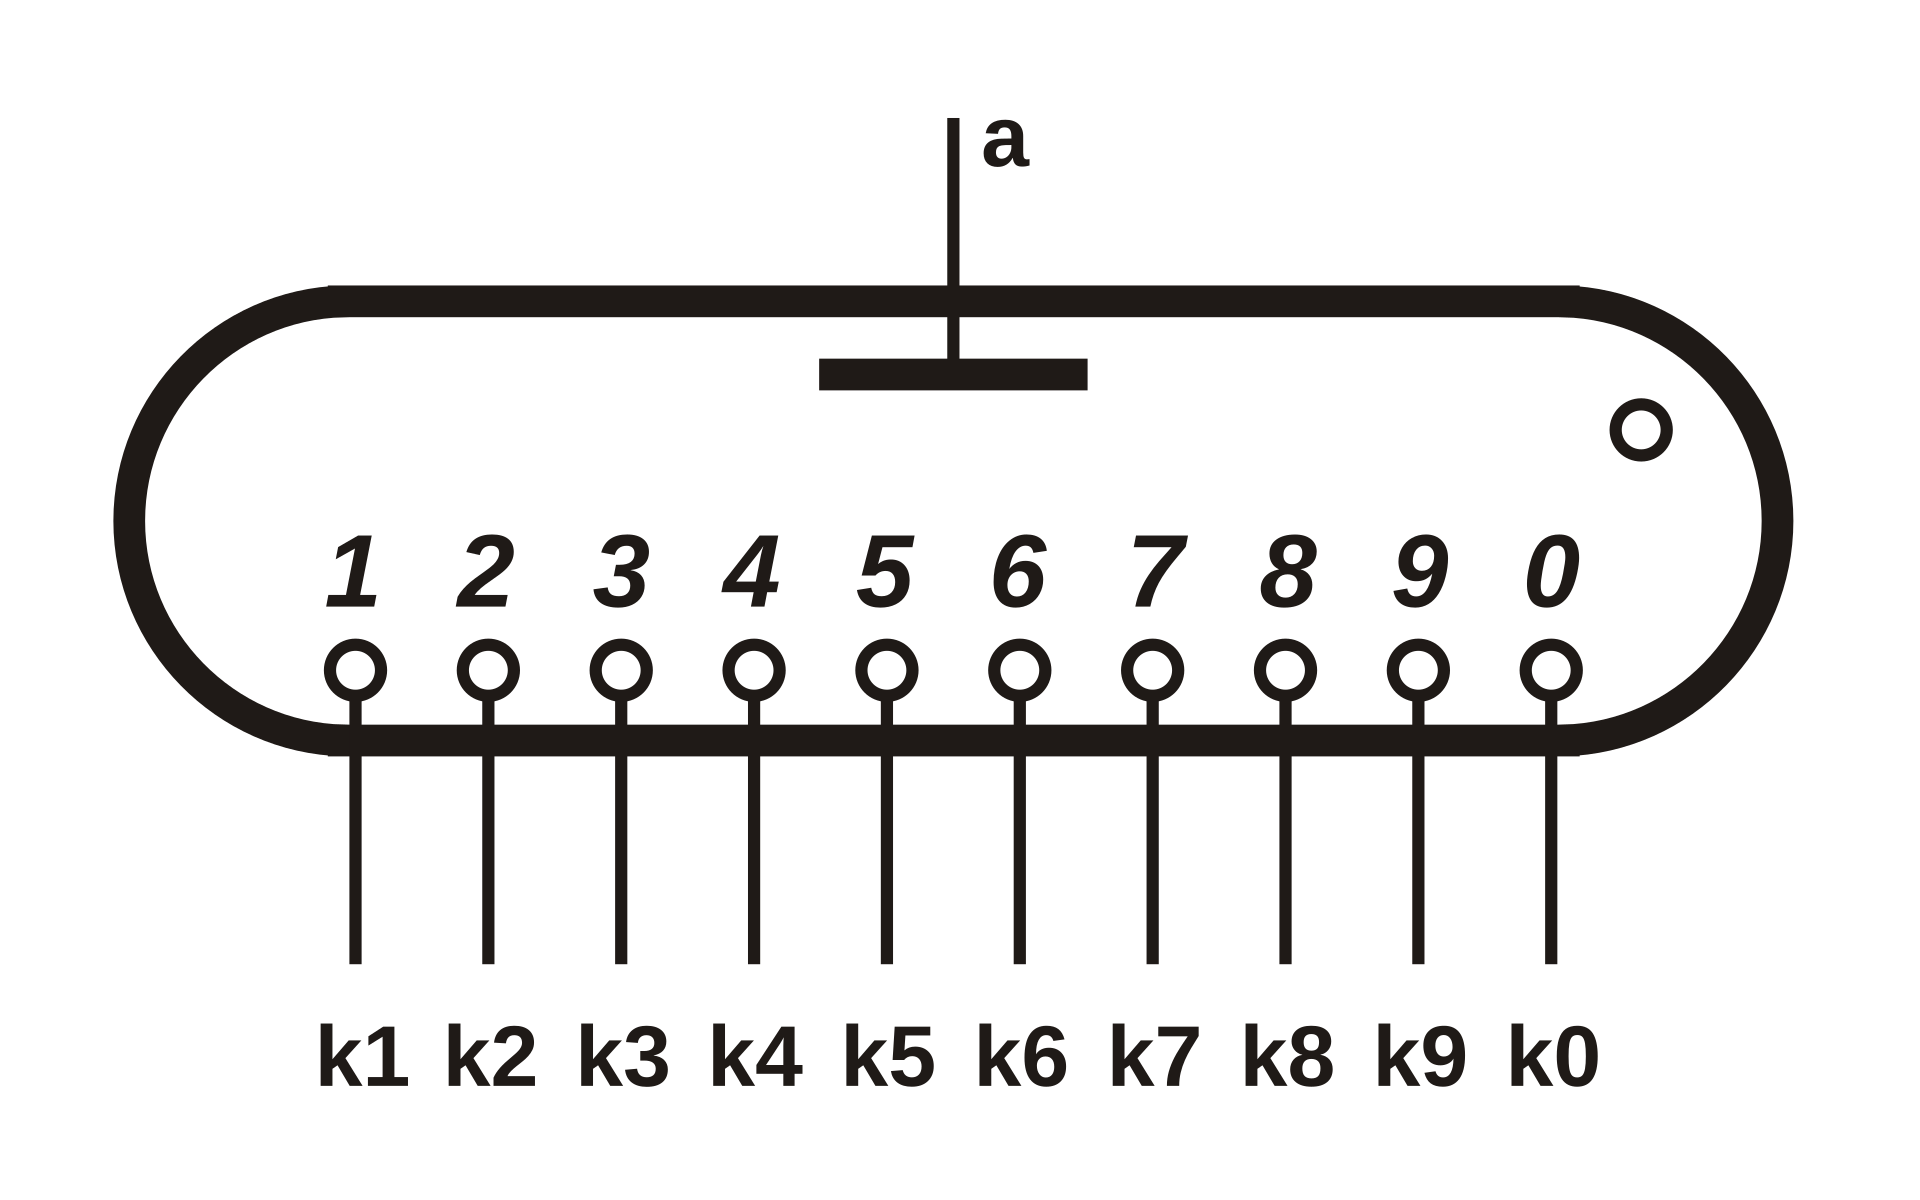
\includegraphics[width=0.5\textwidth]{Nixie_schematic.png}
  \caption{Schemat elektryczny lampy Nixie ze wspólną anodą \cite{st:nixie-jpg}. a - anoda, $k_{n}$ - katoda, n - numer katody.}
  \label{fig:nixie_schematic}
\end{figure}

\subsection{Problemy związane z wykorzystaniem lamp Nixie}

Lampy są podatne na wiele problemów, które mogą wystąpić podczas użytkowania, takie jak:
\begin{itemize}
  \item \textbf{Zatrucie katodowe} - zanikanie wyświetlania cyfr, spowodowane nie pełnym pokryciem katody warstwą gazową.
  \item \textbf{Zjawisko spalania} - zjawisko polegające na spalaniu się katod, spowodowane zbyt dużym prądem płynącym przez katodę.
  \item \textbf{Zjawisko cienia} - zjawisko polegające na wyświetlaniu niebieskiej poświaty, spowodowane zbyt dużym napięciem na anodzie.
  \item \textbf{Zjawisko zaniku} - zjawisko polegające na zanikaniu wyświetlania cyfr, spowodowane zbyt małym napięciem na anodzie.
\end{itemize}

Największym problemem jest zatrucie katodowe, które często pojawia się w zegarach wykorzystujących lampy Nixie.
Tylko parzyste wyświetlacze działają w odpowiednich warunkach, ponieważ używają wszystkich cyfr, 
a więc wszystkie cyfry zużywają się równomiernie.
Problem pojawia się w przypadku nieparzystych katod, gdzie niektóre cyfry są używane znacznie rzadziej niż inne.

Na przykład, lampa po skrajnej lewej stronie wykorzystuje cyfry 0, 1, 2 do wyświetlania części dziesiętnej godziny.
Trzecia lampa (pozycja dziesiątek minut) używa cyfr 0, 1, 2, 3, 4, 5. Gdy konkretna cyfra nie jest używana przez długi czas
 (np. cyfra 8 na najbardziej po lewej stronie lampy),
cyfra ta jest pokryta osadem metalu uwolnionym z innych aktywowanych cyfr.
 Te konkretne cyfry ostatecznie będą miały defekty w świeceniu, jeżeli nie zostaną użyte przez długi czas \cite{st:nixie1}.

\subsection{Rozwiązania problemów związanych z lampami Nixie}
Rozwiązaniem problemu zatrucia katodowego jest sterowanie lampami w taki sposób, aby wszystkie cyfry były używane.
Można to osiągnąć przykładowo poprzez animacje, gdy zmienia się cyfra minut.
Można również w godzinach nocnych przez jakiś czas wyświetlać cyklicznie wszystkie cyfry, aby zminimalizować efekt zatruciu katodowemu.

W celu zwiększenia trwałości lamp można zmniejszyć prąd pracy lampy. Ogranicza to
 zjawisko spalania katod, natomiast prąd musi być wystarczająco duży aby lampa świeciła jasno.

\subsection{Sterowanie lampami}
\label{sec:sterownie_lampi}

Sterowanie lampami Nixie jest wymagającym zadaniem ze względu na konieczność zastosowania wysokiego napięcia, co nie
pozwala na sterowanie lampami bezpośrednio z mikrokontrolera bez dodatkowych elementów.
Przy szacowaniu potrzebnych wyprowadzeń mikrokontrolera i elementów założono użycie 6 lamp Nixie, każda lampa ma 10 katod z cyframi od 0 do 9 oraz 
kropkę dziesiętną, co daje 11 sygnałów sterujących na lampę.
Istnieje kilka sposobów sterowania lampami Nixie \cite{st:nixie1}:

\begin{itemize}
    \item Sterowanie bezpośrednie - każda lampa jest sterowana osobno, wykorzystując tranzystor wysokiego napięcia wysterowany przez mikrokontroler.
    Wadą jest konieczność posiadania wielu pinów GPIO, co implikuje zastosowanie mikrokontrolera o dużych gabarytach lub dodatkowe moduły rozszerzeń GPIO. Sumarycznie wymaga to 66 pinów GPIO oraz 66 tranzystorów wysokiego napięcia.
    Można by w tym porzadku zastosować multipleksery co zmniejszyłoby ilość wymaganych pinów GPIO do 16, ale zwiększyło skomplikowanie układu.
    \item Wykorzystanie dedykowanych driverów - istnieją specjalne układy scalone, które są przeznaczone do sterowania lampami nixie,
    wymagają po 4 GPIO na każdą lampę, co daje łącznie 24 potrzebne wyprowadzenia.
    \item Multiplexing - katody każdej lampy są podłączone do jednego drivera, który wybiera katodę i załącza odpowiednią anodę. 
    Wymaga to mniej pinów GPIO bo tylko 10, ale multipleksacja powoduje szybsze zużycie lamp i pojawienie się artefaktów.
    \item Rejestr przesuwny wysokiego napięcia - rozwiązanie wymaga tylko 3 pinów GPIO. Rejestry wysokiego napięcia są ciężko dostępne i drogie.
    Rejestry muszą posiadać zatrzask. Wymagane jest również by rejestry miały wyjścia typu Open Drain.
    \item Połączenie rejestrów przesuwnych z driverami - połączenie rejestrów przesuwnych wysokiego napięcia z dedykowanymi driverami, pozwala na zastosowania
    rejestru przesuwnego na niskie napięcie. Ta kombinacja również wymaga 3 pinów GPIO, przy rejestrze 32 bitowym i 6 driverach. Powoduje jednak to
    większe skomplikowanie układu oraz wzrost objętości zajmowanego miejsca.
\end{itemize}
Podsumowanie przedstawiono w tabeli \ref{tab:tabela_oplacalnosci}.
%tabela opłacalności czyli : nazwa, ilość pinów, cena, trudność w implementacji, zajętość miejsca
\begin{table}[H]
  \centering
  \begin{tabular}{|c|c|c|c|c|}
    \hline
    Nazwa & Ilość pinów & Cena & Trudność implementacji & Objętość\\
    \hline
    Sterowanie bezpośrednie & 66 & niska-średnia & niska-średnia & duża \\
    \hline
    Multiplexing & 10 &niska & wysoka & mała \\
    \hline
    Dedykowane drivery & 24 &średnia & niska & średnia \\
    \hline
    Rejestr przesuwny HV & 3 &wysoka & niska & średnia \\
    \hline
    Rejestr przesuwny + drivery & 3 & wysoka & średnia & duża \\
    \hline
  \end{tabular}
  \caption{Tabela opłacalności sposobów sterowania lampami Nixie}
  \label{tab:tabela_oplacalnosci}
\end{table}

\subsection{Sytuacja na rynku}
Obecnie dostępność lamp Nixie jest ograniczona, gdyż nie są one już produkowane masowo. Istnieją małe firmy, które zajmują się produkcją, ale są to bardzo
duże lampy w małych ilościach, co powoduje ich wysoką cenę. Dostępne są również lampy używane, ale w tym przypadku również duże lampy są drogie, a małe lampy są trudne do znalezienia.
Problemem jest również niewiadomy stan lamp, ponieważ są to produkty w większości używane.

\end{document}
